\documentclass{article}
\usepackage{amsmath, amssymb, IEEEtrantools}
\usepackage{amsthm}
\usepackage{graphicx}
\usepackage{array}

\title{Representation of Mathematical Expressions in \LaTeX}
\author{Simon Xiang}
\date{\today}
\theoremstyle{definition}
\newtheorem{definition}{Definition}

\begin{document}
\begin{titlepage}
    \begin{center}
        \vspace*{1cm}
 
        \Huge
        \textbf{Experiment 5: Friction and the Inclined Plane}
 
        \vspace{0.5cm}
        \LARGE
        PHYS LAB 1730
 
        \vspace{1.5cm}
 
        \textbf{Simon Xiang}
 
        \vfill
  
        \vspace{0.8cm}
 
        \Large
        Physics Lab Section 518\\
        University of North Texas\\
        \today
 
    \end{center}
\end{titlepage}

\section{Abstract}
The objective of this experiment was to experimentally determine the coefficient 
of friction between two surfaces using two different methods, and find out what 
factors lead to the determination of such friction coefficient. Some of the factors
included mass of the object, angle of elevation, and the surface area of the object
in contact with the plane. The two methods used included adding weights to a pulley 
until the tension force from the pulley overcame the static friction of a weighted
block on a flat surface, and adding weights to a pulley until it overcame the static
friction of an unweighted block on an inclined surface. Throughout both of these 
methods, the factors mentioned above were all varied to ensure consistent results.

In our results, we found that the experimental values determined for the 
coefficient of kinetic friction were mostly consistent with one another. There were small
lapses in between the experimental values, due to factors such as human error in 
the stopwatch timing, judgmental errors in determining the amount of weight needed
to overcome the static friction force, and inconsistencies between the surfaces 
and blocks themselves. This ultimately means that factors such as mass, angle, and surface area
ultimately have a negligible effect on the kinetic friction coefficient.
\section{Introduction}
The coefficient of kinetic friction is a constant that depends on the two
surfaces that it relates. Friction is a force that acts against the movement
of an object on a surface. Two major types of friction forces include static friction
and kinetic friction. Static friction is the force of friction when an object
is at rest, and kinetic friction is the force of friction when an object is in
motion. The force of static friction is always larger than the force of 
kinetic friction, which is why the experiment involves giving the block a "push"
to overcome the force of static friction and set the object into motion, allowing
for the measurement of the coefficient of kinetic friction. The coefficient of 
kinetic friction is simply the the ratio of the force of kinetic energy to the 
normal force. Since it compares two forces whose units are both in Newtons, it is dimensionless. It is given by 
the equation
\begin{equation} \label{eq:1}
    \mu_k = \frac{F_k}{N},
\end{equation}
where $\mu_k$ is the coefficient of kinetic friction, $N$ is the normal force, 
and $F_k$ is the force of kinetic friction. To see where this equation comes from,
consider the equation for the force of kinetic friction, given by
\begin{equation} \label{eq:2}
    F_k=\mu_k N.
\end{equation}
Right multiplying by the multiplicative inverse of $N$ will yield $\mu_k = \frac{F_k}{N}$.
Similarly, consider the equation for the force of static friction, given by
\begin{equation} \label{eq:3}
    F_s=\mu_s N,
\end{equation}
where $F_s$ is the force of static friction, $\mu_s$ is the coefficient of static friction,
and N is the normal force.
Once again, right multiplication by the inverse of N will yield
\begin{equation} \label{eq:4}
    \mu_s = \frac{F_s}{N},
\end{equation}
which is the equation for the coefficient of static friction. 
\begin{figure}
    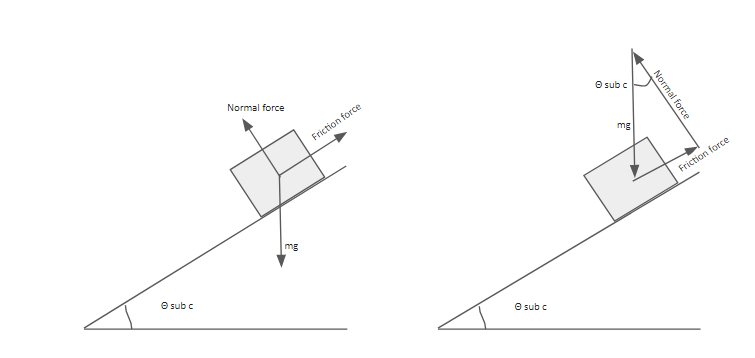
\includegraphics[width = 1 \columnwidth]{fig1.PNG}
    \caption{The free body diagram.}
    \label{fig:1}
\end{figure}
In the case of an inclined plane, the equations for the normal force and the kinetic friction can 
be given by
\begin{equation} \label{eq:5}
    F_k = mg \sin (\theta_c)
\end{equation}
and
\begin{equation} \label{eq:6}
    N = mg \sin (\theta_c),
\end{equation}
where $m$ is the mass of the object in kg, $g$ is the gravitational constant in
$\frac{cm}{s}$, and $\theta_c$ is the angle between the ground and the inclined 
plane. The gravitational force is measured in $\frac{cm}{s}$ because all forces
in this experiment were calculated in dynes, where $1 \, \text{dyn} = 1 \, \frac{g\cdot cm}{s^2}$
. Therefore, $g = 980 \, \frac{cm}{s}$. Since $\mu_k = \frac{F_k}{N}$, we simply
divide equation \ref{eq:5} by equation \ref{eq:6} to obtain
\begin{equation}\label{eq:7}
    \mu_k = \frac{F_k}{N} = \frac{mg \sin (\theta_c)}{mg \sin (\theta_c)} =
    \tan (\theta_c).
\end{equation}
These equations can be obtained from the free body diagram as shown in Figure
 \ref{fig:1}. By the right triangle in the right half of  Figure \ref{eq:1}, 
 we can see that $\sin(\theta_k) = \frac{F_k}{mg}$ and
$\cos(\theta_k) = \frac{N}{mg}$. We can easily rearrange these expressions to obtain equations
\ref{eq:5} and \ref{eq:6}.
\newpage
\section{Apparatus}
The apparatus used are listed below: 
\begin{itemize}
    \item Adjustable inclined plane
    \item Wooden block with holes on side and top
    \item Varying weights of grams (including 500g and 1kg)
    \item Hanger for the weights
    \item String with a length of one meter
    \item Meterstick.
\end{itemize}
The purpose of the experiment was to measure the friction coefficient between the materials
of the surfaces of the block and the inclined plane, making them essential apparatus to the
experiment. The varying weights of grams were attached to the hanger to obtain a precise 
weight at which the block would begin to slide toward the edge on the inclined plane. The 500g
and 1kg gram weights in particular were placed in the holes of the wooden block to increase
its mass. The string was used to connect the block and the weight hanger. Finally, the meterstick was used
in measuring the heights and lengths of the plane.
\section{Experimental Procedure}
\subsection*{Part A}
\begin{enumerate}
    \item Use a triple beam balance to obtain the mass of the block. Use such mass to solve for the weight in dynes, and record the resulting data.
    \item Lay the block down flat on the incline plane with an angle of $0^{\circ}$. Adjust the plane so that the pulley extends beyond the table, allowing for the weight hanger to fall below the table.
    \item Set the height of the pulley and the elevation of the block equal to each other.
    \item Slowly add weights to the weight hanger in small increments, testing to see if the weight is enough to overcome the force of kinetic friction each time by giving the block a small push to overcome the force of static friction.
    \item Record the masses of the weights (including the weight hanger) that overcame the force of kinetic friction successfully.
    \item Add a 500g weight to the block itself. The block should have a hole that fits the 500g weight on both its side and top. Repeat steps 2-5. 
    \item Remove the 500g weight and add the 1kg weight. Repeat steps 2-5.
    \item Lay the block on its side, decreasing the surface area in contact with the plane, and repeat steps 2-7.
    \item Raise the incline plane to an angle of $15^{\circ}$. Lay the block down flat on the place, and perform step 4 again.
    \item Repeat step 9 twice, raising the plane to angles of $30^{\circ}$ and $45^{\circ}$ respectively.
\end{enumerate}
\subsection*{Part B}
\begin{enumerate}
    \item Lay the block down flat on the incline plane with a starting angle of $0^{\circ}$. Slowly adjust the angle of the incline plane upward until the block begins to slide down the plane by itself after having received a small push to overcome the force of static friction.
    \item Record the exact angle at which the block was able to successfully overcome the force of kinetic friction. Using the meterstick, obtain the measurements for the height and base (or length) of the plane, and record.
    \item Repeat steps 1 and 2 twice, adding a 500g and 1kg weight to the block each time, respectively. Remove the 500g weight before adding the 1kg weight on the third trial. 
\end{enumerate}
\section{Data}
\textbf{Table 1}: Data obtained from steps 1-8 of part A.
\begin{center}
    \begin{tabular}{|m{5em} | m{1.9cm} | m{1cm} | m{1cm} | m{2.05cm} | m{1.8cm}|} 
    \hline
    Object moved & Weight W(dynes) & Side Used & Angle ($\theta$) & Pulling Force F(dynes) & Coefficient of Friction\\ 
    \hline\hline
    Block only & $1.92 \cdot 10^5$ & Wide & 0 & $4.90 \cdot 10^4$ & 0.255 \\ 
    \hline
    Block+500g & $6.82 \cdot 10^5$ & Wide & 0 & $1.62 \cdot 10^5$ & 0.251 \\ 
    \hline
    Block+1kg & $1.17 \cdot 10^6$ & Wide & 0 & $2.99 \cdot 10^5$ & 0.256 \\ 
    \hline
    Block only & $1.92 \cdot 10^5$ & Narrow & 0 & $5.39 \cdot 10^4$ & 0.280 \\ 
    \hline
    Block+500g & $6.82 \cdot 10^5$ & Narrow & 0 & $1.79 \cdot 10^5$ & 0.263 \\ 
    \hline
    Block+1kg & $1.17 \cdot 10^6$ & Narrow & 0 & $3.04 \cdot 10^5$ & 0.260 \\ 
    \hline
   \end{tabular}
\end{center}
\newpage
\textbf{Table 2}: Data obtained from steps 9 and 10 of part A. Note that $N =$ Normal Force
$= W\cos\theta$, Parallel Force $= W\sin\theta$, Frictional Force $= f = F - W\sin\theta$, and
the Coefficient of Friction $= \mu_k = \frac{f}{N}$. 
\begin{center}
    \begin{tabular}{|m{4em} | m{1.5cm} | m{0.8cm} | m{1.3cm} | m{1.3cm} | m{1.4cm} |m{1.7cm}|} 
    \hline
    Object moved & Pulling Force F(dynes) & Angle ($\theta$) & Normal Force & Parallel Force & Frictional Force & Coefficient of Friction\\ 
    \hline\hline
    Block only & $9.99 \cdot 10^4$ & $15^\circ$ & $1.86 \cdot 10^5$ & $4.98 \cdot 10^4$ & $5.01 \cdot 10^4$ & 0.269\\ 
    \hline
    Block only & $1.42 \cdot 10^5$ & $30^\circ$ & $1.67 \cdot 10^5$ & $9.62 \cdot 10^4$ & $4.59 \cdot 10^4$ & 0.276\\ 
    \hline
    Block only & $1.68 \cdot 10^5$ & $45^\circ$ & $1.36 \cdot 10^5$ & $1.30 \cdot 10^5$ & $3.16 \cdot 10^4$ & 0.232\\ 
    \hline
   \end{tabular}
\end{center}
\textbf{Table 3}: Data obtained from part B of the experiment. Note that $h$ denotes height
of the inclined plane and $b$ denotes the length of the base of the inclined plane. Also note 
that $\mu_k$ can be calculated two ways, with the respective method for calculating $\mu_k$ listed as the column title. 
\begin{center}
    \begin{tabular}{|m{4em} | m{1.5cm} | m{0.8cm} | m{1.3cm} | m{1.3cm} | m{1.4cm} |m{1.7cm}|} 
    \hline
    Object moved & Weight W(dynes) & Angle ($\theta$) & $h$ (cm) & $b$ (cm) & $\mu_k = \frac{h}{b}$ & $\mu_k = \tan\theta$\\ 
    \hline\hline
    Block only & $1.92 \cdot 10^5$ & $13.5^\circ$ & $16.7$ & $69.8$ & $0.239$ & 0.240\\ 
    \hline
    Block +500g & $6.82 \cdot 10^5$ & $13.5^\circ$ & $16.7$ & $69.8$ & $0.239$ & 0.240\\ 
    \hline
    Block +1kg & $1.17 \cdot 10^6$ & $13.5^\circ$ & $16.7$ & $69.8$ & $0.239$ & 0.240\\ 
    \hline
   \end{tabular}
\end{center}
\section{Calculations and Graphs}
\subsection*{Part A}
\begin{figure}
    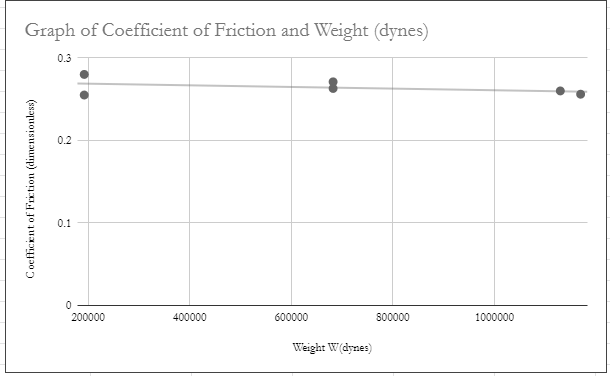
\includegraphics[width = 1 \columnwidth]{fig2.PNG}
    \caption{A plot between $\mu_k$ and $W$(dynes).}
    \label{fig:2}
\end{figure}
Figure \ref{fig:2} details the plot between the coefficient of kinetic friction $(\mu_k)$
and the weight in dynes. A simple linear regression gives a best fit line of
\begin{equation}
    y = (-9.93 \cdot 10^{-9})x + 0.271,
\end{equation}
with
\begin{equation}
    r^2 = 0.194.
\end{equation}
The slope of the line of best fit is negligibly small, yielding a linear equation that
almost seems constant. Therefore, we can conclude that the weight in dynes has a negligible 
effect on the coefficient of kinetic friction. Examining Figure \ref{fig:2} closely, there almost
appear to be two sets of points making one graph, due to the fact that both the 
plots for weights on the wide side and the narrow side are plotted together in Figure \ref{fig:2}.
Refer to the table below for a comparison of the percent differences \footnote{The percent difference between two values, say $x_1$ and $x_2$, is given by
the formula \begin{equation}
    \frac{\mid x_1 - x_2 \mid}{avg(x_1,x_2)} \cdot 100\%,
\end{equation} where $avg(x_1,x_2) = \frac{x_1+x_2}{2}$.}
 between the coefficient of 
kinetic friction determined by the wide side and the narrow side making contact with the inclined plane. 
\begin{center}
    \begin{tabular}{ c | c c c}
      & $\mu_k$ (Wide side) & $\mu_k$ (Narrow side) & Percent difference \\ 
     \hline
     Block only & 0.255 & 0.280 & 9.35\% \\  
     Block + 500g & 0.251 & 0.263 & 4.67\% \\  
     Block + 1kg & 0.256 & 0.260 & 1.55\%  
    \end{tabular}
\end{center}
In the table above, the percent differences between the values obtained through placing the 
block on its wide side and placing the block on its narrow side are extremely low.
Therefore, we can conclude that both weight and surface area are negligible in the
calculation of the coefficient of kinetic friction, due to the extremely small coefficient 
of the linear line of best fit generated by linear regression and the extremely low percent 
differences obtained by comparing the values of $\mu_k$ for the wide and narrow sides of the block.

Let us turn our attention to Figure \ref{fig:3}. This details the plot between the 
angle of incline of the inclined plane, $\theta$, and the coefficient of kinetic friction,
$\mu_k$. In this graph, $\mu_k$ was measured with three different values of $\theta$,
the values being $15^\circ, 30^\circ,$ and $45^\circ$ respectively. Once again performing a simple
linear regression on Figure \ref{fig:3}, we obtain
\begin{equation}
    y = (-1.23 \cdot 10^{-3})x + 0.296
\end{equation} 
as the line of best fit, and
\begin{equation}
    r^2 = 0.612.
\end{equation}
Once again the linear coefficient of the line of best fit is negligibly small, and we 
can safely conclude that $\theta$ does not have any substantial impact on $\mu_k$.
\begin{figure}
    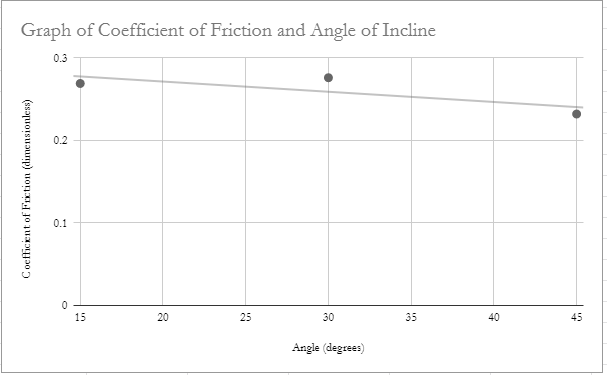
\includegraphics[width = 1 \columnwidth]{fig3.PNG}
    \caption{A plot between $\mu_k$ and $\theta$ (angle of incline).}
    \label{fig:3}
\end{figure}
\subsection*{Part B}
In this part of the experiment, we measured the angle at which the block (at varying weights)
would begin to slide down the inclined plane. Since we obtained the exact same values of theta 
($\theta = 13.5^\circ$) for all 
three weights of the block (no weight, +500g, +1kg), $\mu_k$ almost didn't change at all
with the varying weights. We present the percent differences of $\mu_k$ calculated two ways below:
\begin{center}
    \begin{tabular}{ c | c c c}
      & $\mu_k = \frac{h}{b}$ & $\mu_k  = \tan\theta$ & Percent difference \\ 
     \hline
     Block only & 0.239 & 0.240 & 0.42\% \\  
     Block + 500g & 0.239 & 0.240 & 0.42\% \\  
     Block + 1kg & 0.239 & 0.240 & 0.42\%,
    \end{tabular}
\end{center}
where the first value of $\mu_k$ was calculated by dividing $h$, the height in centimeters
of the inclined plane by $b$, the length of the base of the inclined plane in centimeters.
The second value of $\mu_k$ was calculated by taking the tangent of the angle of incline 
of the inclined plane $(\theta)$. As can be seen by the astronomically low percent difference, 
the effect of the weight of the block on the coefficient of kinetic friction is truly negligible.
\section{Discussion of Results and Error Analysis}
The purpose of this experiment was to obtain the coefficient of kinetic friction between two
surfaces, and measure the impact of various factors on the determination of such coefficient of 
kinetic friction. Since the value of $r^2$ was low for both linear regressions of Figure \ref{fig:2}
and Figure \ref{fig:3}, there doesn't appear to be much of a correlation between the weight of 
the object and the angle of incline of the inclined plane $(\theta)$ with the coefficient of kinetic friction
$(\mu_k)$, respectively. On the topic of surface area, the percent difference between the values of
$\mu_k$ obtained by using the wide and narrow sides of the block respectively were extremely small, 
leading to the conclusion that the amount of surface area of the object in contact with the inclined plane
is not relevant to the value of the coefficient of kinetic friction either.
Therefore, we can safely conclude that $\mu_k$ is independent of external factors 
such as weight, angle of incline, or surface area. 

However, even though the percent differences were extremely low, there were still differences between
the values calculated as the methods changed. Some reasons for this difference include the method
of calculation, namely the difference between analytical and experimental methods of obtaining the value of
$\mu_k$. For example, consider the two methods for calculating $\mu_k$ in Part B, namely
\begin{equation}
    \mu_k = \frac{h}{b}
\end{equation} 
and 
\begin{equation}
    \mu_k  = \tan\theta
\end{equation}
respectively. Equation 13 is more susceptible to measurement error since it requires taking the measurements
of the height and base of the inclined plane, the measurements for which may be to the slightest degree 
inaccurate due to the fact that the meterstick's resolution is not high enough. On the other hand, 
Equation 14 only relies on the angle $\theta$, which is still prone to error, but on a smaller scale, since only
one variable depends on the resolution of the instrument used.

There were several other factors that may have led to the percent differences between the trials. 
The inclined plane was not completely even, leading to blocks sliding down with different masses depending
on which part of the plane it was placed on. Judgmental lapses may have led to recording an inaccurate value 
for the weight required for the block to overcome the force of kinetic friction. For example, if the weight was recorded
after pushing the block and prematurely stopping it due to the assumption that it had already overcome kinetic friction, it would be incorrect since the
block was really only moving due to the fact that it was set in motion by the initial push.
\section{Conclusion}
Concluding the experiment, the outcome of the experiment strongly supports the theory proposed that the
coefficient of kinetic friction is not dependent on outside factors. With the highest percent difference between
different surface areas being $9.35\%$ and the highest percent difference between the angles being
$0.42\%$, it is clear that such factors are not important factors in determining $\mu_k$.

Some ways that the error could be reduced include obtaining an instrument with a higher resolution to measure certain
measurements such as the degree of $\theta$ and the values of $h$ and $b$. Another way to reduce the error includes 
using newer surfaces for the incline plane and blocks, since the older ones tend to accumulate debris that impacts the 
friction between the two surfaces. Finally, using smaller increments to measure the exact gram weight at which the block 
overcomes the force of kinetic friction would lead to a more precise value for the weight, improving the accuracy of the 
experiment. Implementing these methods would surely reduce the percent difference, and perhaps even eliminate the
difference altogether.

\end{document}